\documentclass[a4paper]{article}

\usepackage[hidelinks]{hyperref}
\usepackage[notquote]{hanging}
\usepackage{siunitx}
\usepackage{amsmath}
\usepackage[margin=1in]{geometry}
\usepackage{pgfplots}
\pgfplotsset{width=10cm, compat=newest}
\usepackage{setspace}
\usepackage{listings}
\usepackage{graphicx}
\usepackage{subcaption}
\usepackage{csvsimple}
\usepackage{supertabular}
\usepackage{booktabs}
\usepackage{multicol}
\setlength{\columnsep}{3cm}

\newcount\n
\n=0
\def\tablebody{}
\makeatletter
\loop\ifnum\n<100
        \advance\n by1
        \protected@edef\tablebody{\tablebody
                \textbf{\number\n.}& shortText
                \tabularnewline
        }
\repeat

\makeatletter
\let\mcnewpage=\newpage
\newcommand{\TrickSupertabularIntoMulticols}{%
  \renewcommand\newpage{%
    \if@firstcolumn
      \hrule width\linewidth height0pt
      \columnbreak
    \else
      \mcnewpage
    \fi
  }%
}
\makeatother

\begin{document}
\title{Investigating the effects acting upon a rapidly rotating wheel free to
rotate around all three dimensions}
\author{}
\date{}

\maketitle

\onehalfspacing

\section*{Rationale}

\paragraph*{}
My passion in physics is electronics. Perhaps a passion since young age,
perhaps something related to my love for computers - in any case, a love for
electronics is present. I sincerely and truly enjoy everything related from the
basics of electronics to the complexities of processing signals. Naturally, I
decided that I would do my physics internal assessment in the field of
electronics. My original idea was to measure the frequency response of a
commonly available signal boost pedal, the \textit{MXR Microamp}. However, my
original idea was rejected due to being out of syllabus.

\paragraph*{}
I needed a new topic, and since I have a burning passion for engineering in
general, as well as electrical engineering, I decided to look into physical
phenomena that intrigue me. On one day I was riding a bicycle when I realized
what my topic could be - spinning wheels. I always found the motion of wheels
to be somewhat unintuitive, so I decided to challenge myself by doing my
internal assessment on them.

\section{Introduction}

\paragraph*{}
Unlike point masses, actual bodies can be rotated, and, as such, these bodies
exhibit certain properties that point masses do not posses. A comparison
between a point mass and a physical body is shown in figure
\ref{fig:pm-rb-comparison}.

\begin{figure}[ht]
  \centering
  \begin{tikzpicture}
    \draw (-2,0) node[circle,fill,inner sep=1pt,label=below:$A$](A){};
    \draw [red] (1,0) circle (1);
    \draw (1,0) node[circle,fill,inner sep=1pt,label=below:$B$](B){};
  \end{tikzpicture}
  \caption{A comparison between a point mass and a physical body}
  \label{fig:pm-rb-comparison}
\end{figure}

\paragraph*{}
Let us consider these objects when equal forces are applied:

\begin{figure}[ht]
  \centering
  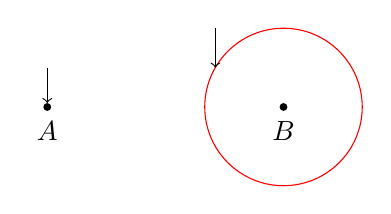
\begin{tikzpicture}
    \draw (-2,0) node[circle,fill,inner sep=1pt,label=below:$A$](A){};
    \draw [red] (1,0) circle (1);
    \draw (1,0) node[circle,fill,inner sep=1pt,label=below:$B$](B){};
    \draw [->] (-2, 0.5) -- (-2,0.05);
    \draw [->] (0.13397, 1) -- (0.13397,0.5);
  \end{tikzpicture}
  \caption{A comparison between a point mass and a physical body when forces
  are applied}
\end{figure}

\paragraph*{}
Whenever a linear force is applied to a point mass, it will always create an
acceleration proportional to the force and inversely proportional to the
inertivity of the object:
$$
\vec{a} = \frac{\vec{F}}{m}
$$

\paragraph*{}
However, for a real object, whenever a linear force is applied in a line which
does not intersect with the centre of mass of the object, the object will
rotate. At a given moment, the linear force can be calculated by separating the
force vector into two vectors, one which is colinear with the centre of mass
and one which is tangential to the object's edge.

%\begin{figure}[ht]
%  \centering
%  \begin{tikzpicture}
%    \draw [red] (0,0) circle (1);
%    \draw (0,0) node[circle,fill,inner sep=1pt,label=below:$B$](B){};
%
%    \draw [->] (-0.866, 1) -- (-0.866, 0.5);
%    \draw [->] (-0.866, 1) -- (0, 0);
%
%  \end{tikzpicture}
%  \caption{A comparison between a point mass and a physical body when forces
%  are applied}
%\end{figure}

\paragraph*{}
The vector which is tangential to the object's edge creates a rotational action
upon the object. This rotational action can be measured through torque:
\begin{align*}
  \vec{\tau} &= \vec{F_t} \times \vec{r} \\
  \text{where}~\vec{F_t} & \text{ is the tangential force vector} \\
  \vec{r} & \text{ is the radius vector}
\end{align*}

\subsection{Rotational mechanics}

\paragraph*{}
Torque is analagous to force. It is a measure of the change of angular
momentum, which, for a point mass, is defined analogously to linear momentum
$\left( \vec{L} = m\vec{v} \times \vec{r} = m r \vec{\omega} \times \vec{r} = I
\vec{\omega} \right)$. $I$ is the moment of inertia, defined as $I = m r^2$ for
a point mass revolving around a point with distance $r$ from it. Note that this
definition is somewhat limiting in the sense that it is only true for point
masses (which is meaningless given that linear momentum only has meaning for
non-point objects). The true definition is the sum of all infinitesimally small
individual point masses:
$$I = \iiint m(x, y, z) ||r||^2 dV $$

\paragraph*{}
Torque is, from these definitions:
\begin{align*}
  \vec{\tau} &= \frac{d\vec{L}}{dt} \\
  &= \frac{d (I\vec{\omega})}{dt}
\end{align*}

\paragraph*{}
An inherent property of torque is that, like force, the resulting torque is the
total change in angular momentum:
$$\sum_i \vec{\tau_i} = \frac{d\vec{L}}{dt}$$

\paragraph*{}
These basic principles govern the motion of all physical objects in physical
space.

\subsection{Freewheel mounted on a gimbal}

\paragraph*{}
In this section a freewheel mounted on a gimbal as given in figure
\ref{fig:gimbal-fw} is presented and the actions it undertakes are
mathematically described.

\begin{figure}[ht]
  \centering
  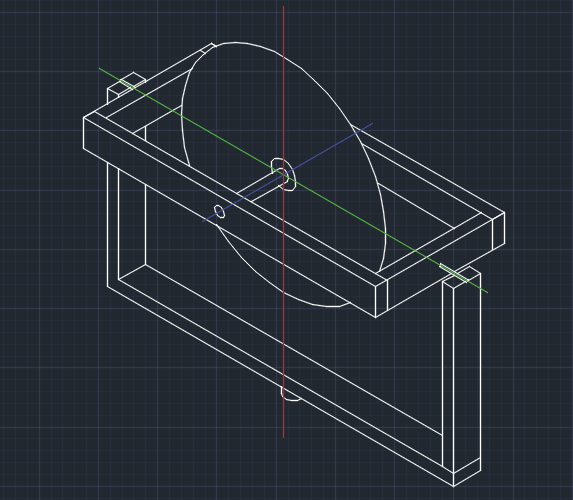
\includegraphics[width=0.5\textwidth]{img/gimbal-fw}
  \caption{A freewheel mounted on a gimbal}
  \label{fig:gimbal-fw}
\end{figure}

\paragraph*{}
Let us take a moment to define the key elements in this setup. The
\textit{freewheel} is a wheel which is rotating around an axis (in figure
\ref{fig:gimbal-fw} the blue $Z$ axis) without any friction. The
\textit{gimbal} is a single element which allows for free rotation. This setup
contains two gimbals - one around the red $X$ axis and the other around the
green $Y$ axis.

\paragraph*{}
Let us define the following:
\begin{align*}
  \vec{r_x} & \text{ - the vector of distance of the $X$ gimbal from the center
  of to the edge}
\end{align*}

\subsubsection{Freewheel not rotating}

\paragraph*{}
To understand the motion of the contraption upon the action of a force
tangential to the $X$ gimbal, let us first consider the case when the wheel is
not spinning. Consider a pulley of mass $m_w$ added at a position away from the
gimbal and connected to its edge with a massless string. For this case, it is
supposed that the distance is high enough such that $\sin(\theta) = \theta$.
Then:
\begin{align*}
  \vec{\tau} &= \vec{F} \times \vec{r_x} \\
  &= m_w \vec{g} \times \vec{r_x} \\
  \vec{\tau} &= I \vec{\alpha} \\
  I \vec{\alpha} &= m_w \vec{g} \times \vec{r_x}
\end{align*}

\paragraph*{}
Note that $I$ is equal to $k m r^2$ and that $k$ is an arbitrary coefficient
which depends on the body that is rotating. Let $m_b$ the mass of the rotating
body. It follows that:

\begin{align*}
  k \cdot m_b r_x^2 \vec{\frac{a}{r_x}} &= m_w \vec{g} \times \vec{r_x} \\
  m_b \vec{a} &= m_w \vec{g} \\
  a &= \frac{m_w}{m_b} \vec{g} \\
  a &= k \vec{g}
\end{align*}

\paragraph*{}
Note how the acceleration is linearly proportional to the acceleration of the
pulley (the gravitational acceleration).

\subsubsection{Freewheel rotating} \label{sec:fw-rotating}

\paragraph*{}
Let us now consider the case of the freewheel rotating and having a certain
angular velocity.

\paragraph*{}
Let the freewheel be spinning around the $Z$ axis in a direction towards the
observer, as shown in figure \ref{fig:gimbal-fw-1}.

\begin{figure}[ht]
  \centering
  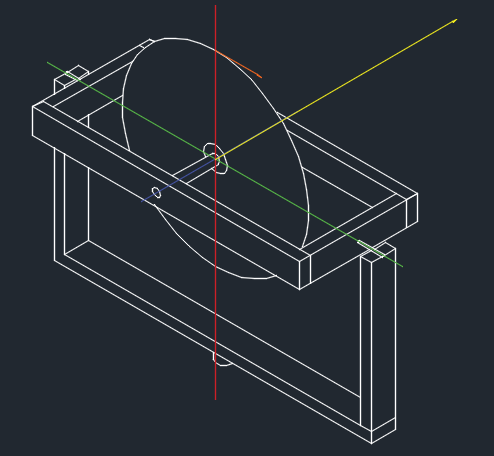
\includegraphics[width=0.4\textwidth]{img/gimbal-fw-1}
  \caption{The spinning freewheel gimbal}
  \label{fig:gimbal-fw-1}
\end{figure}

\paragraph*{}
The vector of angular velocity $\vec{\omega}$ is marked in orange and is
pointed away from the observer. The direction of the angular momentum $\vec{L}$
is the same, therefore, and is marked in yellow. Its magnitude is equal to:
$$\vec{L} = I \vec{\omega}$$

\paragraph*{}
When a force $\vec{F_x}$ (marked in purple) is applied to the device, it
creates a torque $\vec{\tau}$ (marked in pink) pointed parallel to the $Y$ axis
as shown in figure \ref{fig:gimbal-fw-2}.

\begin{figure}[ht]
  \centering
  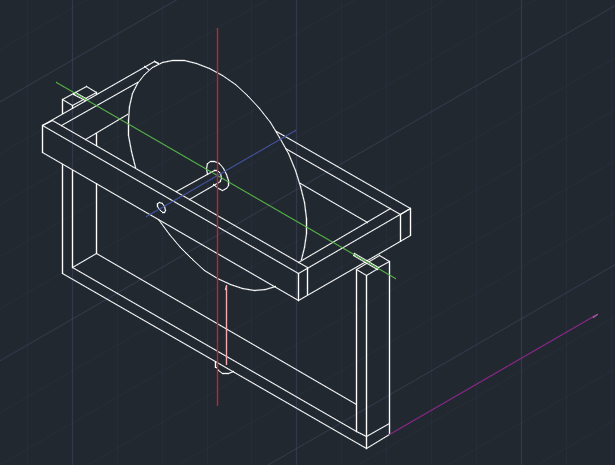
\includegraphics[width=0.4\textwidth]{img/gimbal-fw-2}
  \caption{The spinning freewheel gimbal}
  \label{fig:gimbal-fw-2}
\end{figure}

\paragraph*{}
Note that torque is defined as:
$$\vec{\tau} = \frac{d \vec{L}}{dt}$$
It acts upon the angular momentum. Its action is shown in figure
\ref{fig:gimbal-fw-3}.

\begin{figure}[ht]
  \centering
  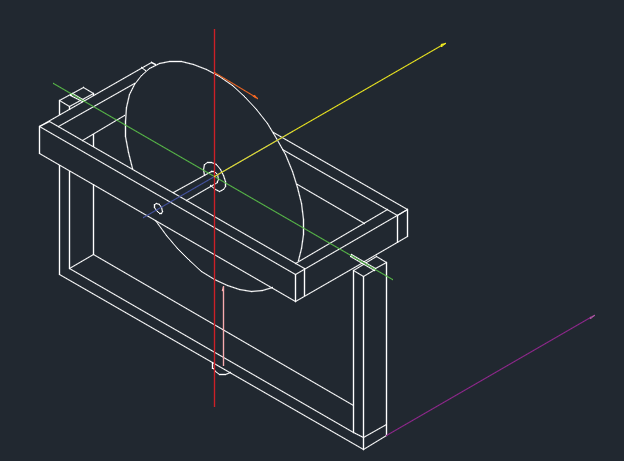
\includegraphics[width=0.4\textwidth]{img/gimbal-fw-3}
  \caption{The spinning freewheel gimbal}
  \label{fig:gimbal-fw-3}
\end{figure}

\paragraph*{}
This action leads to a rotation of the $Y$ gimbal. Let us consider a small
change in $L$, $dL$. The proportional $d \theta$, according to trigonometry,
would be equal to:
$$d \theta = \tan \left( \frac{dL}{L} \right) $$

\paragraph*{}
Since $\theta = \sin \theta = \tan \theta$ at very small angles. We may use
this identity since $dL$ is infinetesimally small. The equation then becomes:
$$d \theta = \frac{dL}{L}$$

\paragraph*{}
Let us define a special kind of angular velocity, the \textit{precession}, as
the change in the angle of rotation of the $Y$ gimbal:
$$\Phi = \frac{d \theta}{dt}$$

\paragraph*{}
With the previously discussed equations, this value becomes:
\begin{align*}
  \Phi &= \frac{d \theta}{dt} \\
  &= \frac{dL}{L} \cdot \frac{1}{dt} \\
  &= \frac{dL}{dt} \cdot \frac{1}{L} \\
  &= \frac{1}{L} \vec{\tau}
\end{align*}

\subsection*{}

\paragraph*{}
According to the aforementioned equations, a freewheel which is not spinning
behaves intuitively. However, when the freewheel is spinning, and a force is
applied to the $X$ gimbal, a motion will emerge in the $Y$ gimbal.

\subsection{Research goal}

\paragraph*{}
The complexity of rotational mechanics has only been hinted at. The field is
yet even more complex than what is hinted at here. To proceed with research,
this paper focuses on the relationship between the velocity of the rotating
wheel and the inclination of the $Y$ gimbal as described in section
\ref{sec:fw-rotating}.

\paragraph*{}
The goal of this research, therefore is to find the empirical relationship
between the angular velocity of the wheel $\omega$ and the angle of inclination of the
$Y$ gimbal $\psi$ upon a force being applied on the $X$ gimbal. The
\textit{independent variable} is the angular velocity of the freewheel, the
\textit{dependent variable} is the angle of inclination of the $Y$ gimbal and
the \textit{controlled variables} were the force with which the $X$ gimbal is
pulled, the time for which that force acts and the mass of the rotating wheel.

\paragraph*{}
It was hypothesized for the relationship between the angle of inclination to be
proportional to $\ln (\omega I)$, as described in the
following set of equations.
\begin{align*}
  \Phi &= \frac{1}{L} \vec{\tau} \\
  &= \frac{1}{\omega I} \frac{dL}{dt} \\
  &= \frac{1}{\omega I} \frac{d(\omega I)}{dt}
\end{align*}

\begin{align*}
  \psi &= \int \Phi dt \\
  &= \int \frac{1}{\omega I} \frac{d(\omega I)}{dt} dt \\
  &= \ln \omega I
\end{align*}

\section{Method}

\subsection{Preparation}

\paragraph*{}
To measure the aforementioned effect, an object as given in figure
\ref{fig:gimbal-fw} was constructed with certain specific modifications to the
original design. The $X$ axis was inserted into a bearing. The $Z$ axis also
was suspended inside a bearing.
On one of the sides of the $Y$ gimbal, a potentiometer was mounted as an axis
for the $Y$ gimbal. This allows for electrically measuring the angle of the $Y$
gimbal. A \textit{reed relay}\footnote{A device which connects two electrical
terminals internally when a magnet is close to the device} was mounted on the
edge of the $Y$ gimbal parallel to the $Z$ axis as shown in figure
\ref{fig:reed}. Small, but powerful, neodymium
magnets were mounted on the wheel. These, when in front of the reed relay,
trigger it, and allow for electrical sensing of the rotation of the wheel.
For higher precission it was decided that $4$ magnets would be used. 

\begin{figure}[ht]
  \centering
  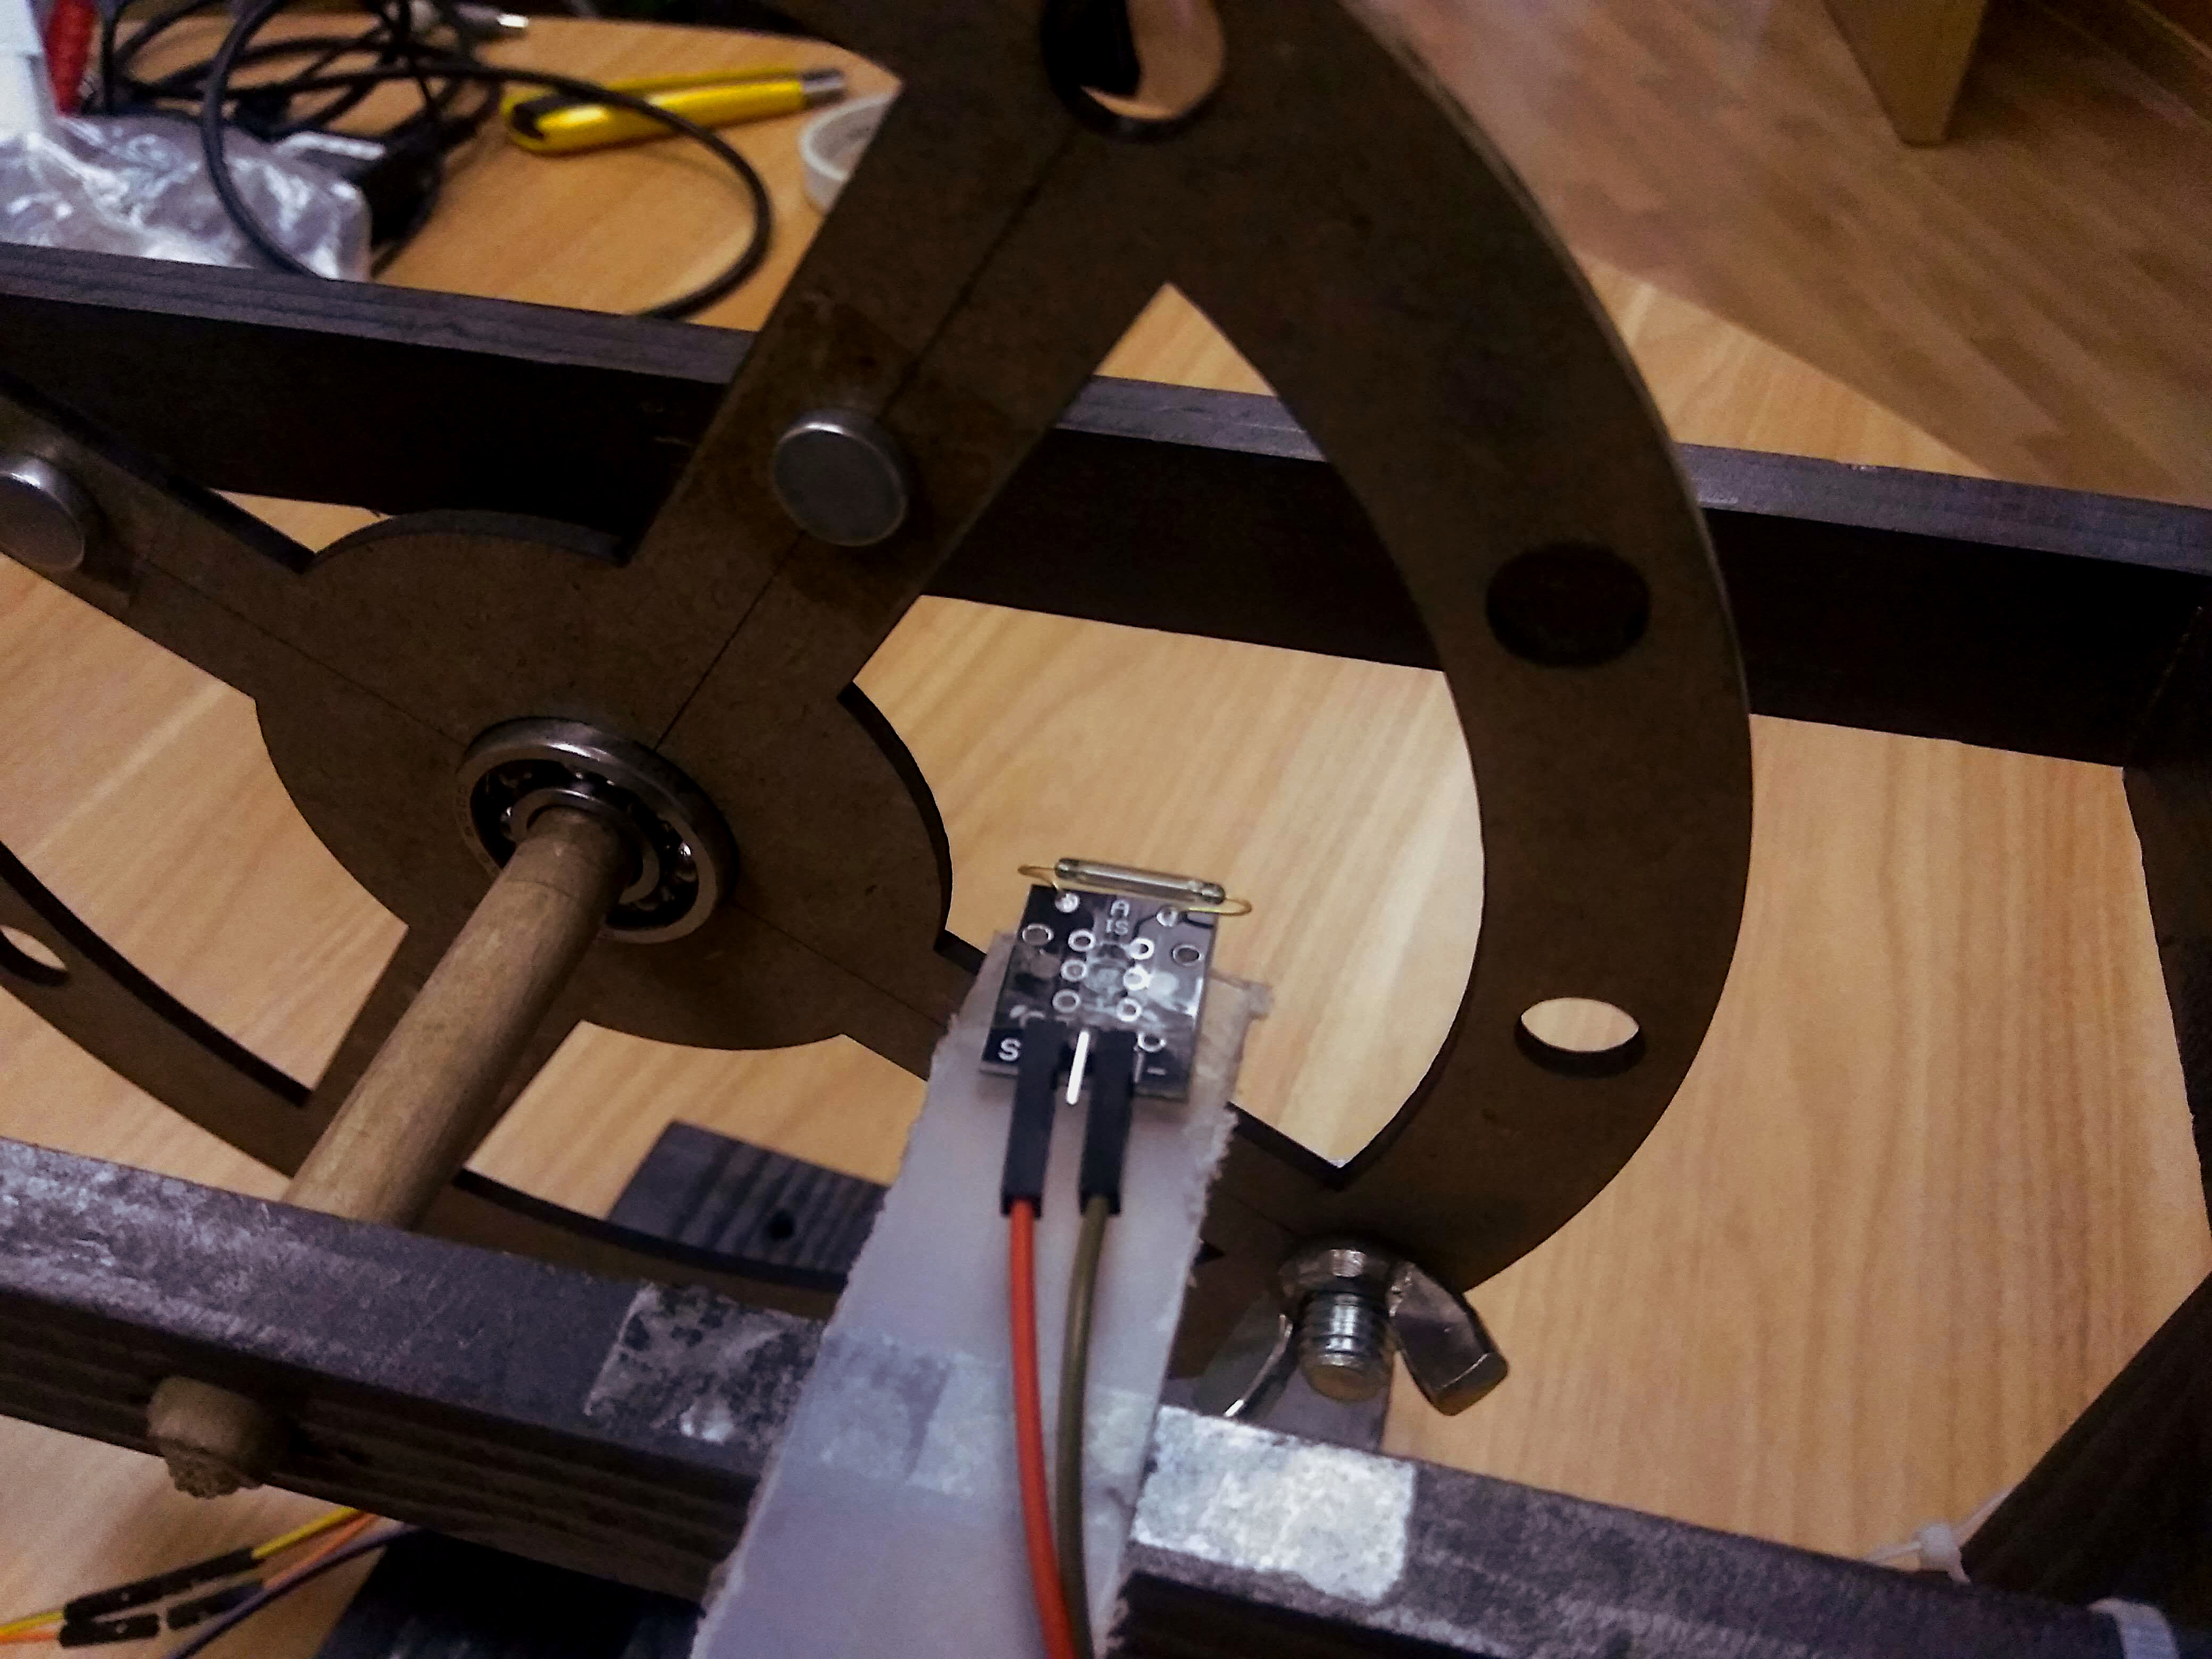
\includegraphics[width=0.6\textwidth]{img/reed}
  \caption{The reed relay}
  \label{fig:reed}
\end{figure}

\paragraph*{}
Electrical connections were established to an \textit{Arduino Uno} (Arduino) as
shown in figure \ref{fig:arduino-schematic}.

\begin{figure}[ht]
  \centering
  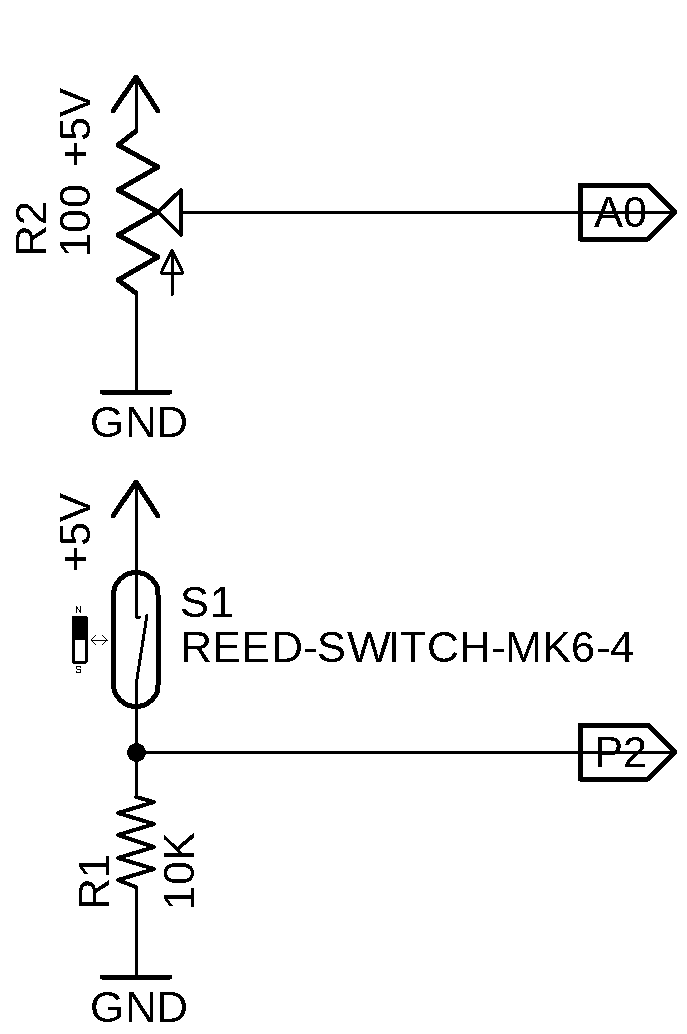
\includegraphics{img/arduino-schematic}
  \caption{The schematic of the electrical connections}
  \label{fig:arduino-schematic}
\end{figure}

\paragraph*{}
The Arduino Uno was programmed to read these values and the code is given in
the appendix. Note how the code utilizes the interrupt service routine to
provide accurate measurements of the angular velocity of the wheel as well as
the angle of inclination.

\paragraph*{}
The setup is shown in figure \ref{fig:setup-whole}.

\begin{figure}[ht]
  \centering
  \includegraphics[width=0.6\textwidth]{img/setup-whole}
  \caption{The setup of the experiment}
  \label{fig:setup-whole}
\end{figure}

\paragraph*{}
Finally, before measurements were done, the pontentiometer angle of rotation
was measured, so as to provide a linear relationship between the resistance of
the potentiometer and the angle of the $Y$ gimbal.

\paragraph*{}
A weight was connected to one edge of the $X$ gimbal over a pulley to ensure a
constant torque acting on the system. Although the force applied was linear,
since the weight was distanced from the contraption, and since $\sin \theta =
\theta$ at low angles, it can be assumed that the torque was constant.

\subsection{Environmental remarks}

\paragraph*{}
Neither the experiment nor the constructed machinery presented any major
environmental impact. The gimbal was constructed from recycled wood to minimize
environmental impact.

\subsection{Experiment conduction}

\paragraph*{}
Upon preparation, the gimbal construction was held in place at an angle of $90
\si{\degree}$ relative to the pulley. The microcontroller was reset and the
following command was immediately run on the machine receiving the data:

\begin{lstlisting}
  cp /dev/ttyACMx Output.csv
\end{lstlisting}
where \textit{x} is the port the microcontroller is connected to.

\paragraph*{}
This command allows for saving the data received from the \textit{Arduino} on a
\textit{Linux} machine.

\paragraph*{}
The wheel was spun by hand and the gimbal was released to be pulled by the
weight. After the gimbal stopped rotating, the copy operation run on the
machine receiving the data was closed by sending an interrupt signal to the
running command (pressing the \textit{CTRL-C} key combination).

\section{Data}

\subsection{Raw data}

\paragraph*{}
The potentiometer maximal rotation was measured to be:
$$\psi_{pot} = (300 \pm 1) \si{\degree} $$

\paragraph*{}
The mass of the weight was measured to be:
$$m_w = (10 \pm 1) \si{g}$$

\paragraph*{}
Since the raw data was collected electronically, it is highly extensive and is
given in the appendix.

\subsubsection{Errors}

\paragraph*{}
The uncertainty of the measurement by \textit{reed relay} was calculated as
follows. Since there are four magnets in a range of $\left[ 0, 2 \pi \right]$,
then it follows that the range of uncertainty is $\left[ 0, \frac{\pi}{2}
\right]$. The distance of this interval is equal to to $\left[ - \frac{\pi}{4}
, + \frac{\pi}{4} \right]$, making the uncertainty:
$$\theta_{error} = \pm \frac{\pi}{4}$$

\subsection{Data processing}

\paragraph*{}
Data processing was done in the \textit{python} programming language (Python
Software Foundation). The script used is given in the appendix.

\subsubsection{Data cleanup}

\paragraph*{}
Due to the na\"{i}ve implementation of the \textit{Arduino} serial code, all
data contained remnants of serial output before the actual data was
transmitted.  Moreover, due to the nature of \textit{UNIX} and \textit{Windows}
line endings, all of the data contained empty \textit{newlines} when copied by
the \textit{cp} command.

\paragraph*{}
The extra line endings where removed with a simple \textit{regex}:

\begin{lstlisting}
^\n
\end{lstlisting}

\paragraph*{}
The remnant data was removed by manually inspecting each individual file and
removing the serial output that was left in the buffer before the restart of
the \textit{Arduino}.

\subsubsection{Graph smoothening}

\paragraph*{}
A graph of the relationship between the time and the angular path is given
in \ref{fig:ang-path-time}, as well as its numerical derivative, the angular
velocity.

\begin{figure}[ht]
  \centering
  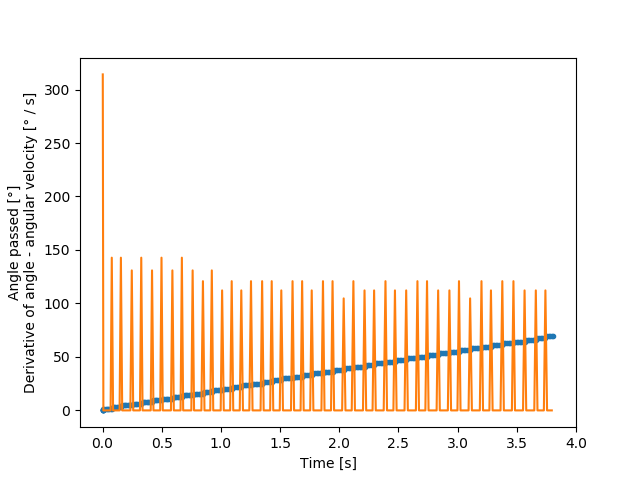
\includegraphics[width=0.7\textwidth]{img/ang-path-time}
    \caption{The relationship between the angular path and the time, including
    the derivative}
  \label{fig:ang-path-time}
\end{figure}

\paragraph*{}
Note how the velocity graph is incorrect. This can be attributed to the fact
that the graph of the angle passed is jagged and is similar to a step function,
as shown in figure \ref{fig:ang-path-time-zoom}.

\begin{figure}[ht]
  \centering
  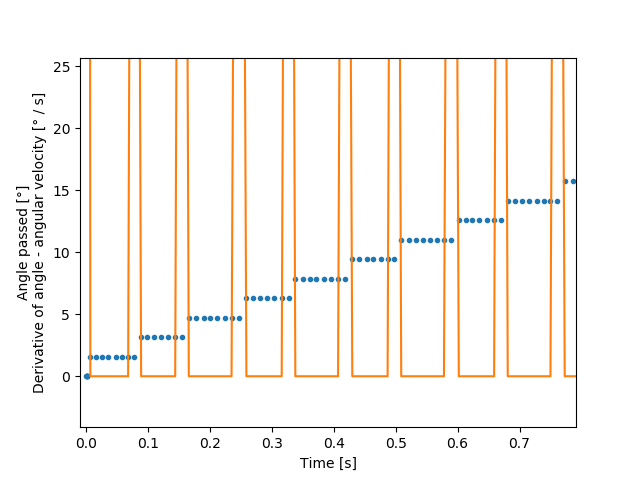
\includegraphics[width=0.7\textwidth]{img/ang-path-time-zoom}
  \caption{Zoomed view of the function given in \ref{fig:ang-path-time}}
  \label{fig:ang-path-time-zoom}
\end{figure}

\paragraph*{}
To resolve this issue, it was necessary to smoothen the graph of the angle
passed. This was achieved by taking the average $x$ coordinate (the time) of
each of the individual data points, where the data points are equal, producing
a graph as given in figure \ref{fig:ang-path-time-fixed}.

\begin{figure}[ht]
  \centering
  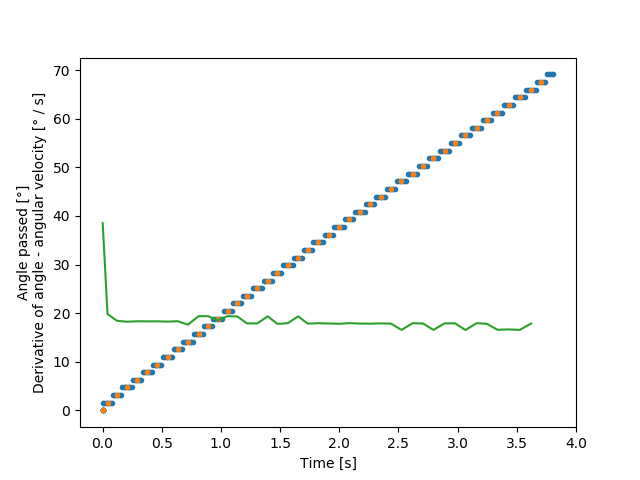
\includegraphics[width=0.7\textwidth]{img/ang-path-time-fixed}
  \caption{The improved graph of figure \ref{fig:ang-path-time}}
  \label{fig:ang-path-time-fixed}
\end{figure}

\paragraph*{}
This results in a more correct function of angular velocity.

\subsubsection{Angular velocity versus the angle of inclination}

\paragraph*{}
With the function of the angular velocity calculated, it was possible to
calculate the relationship between the initial velocity of the wheel and the
angle of inclination.

\paragraph*{}
Since there was certain error (as shown in figures \ref{fig:v-theta-4} and
\ref{fig:v-theta-2}) in the calculation of the angular velocity, it was decided
that the average of the angular velocity would be taken rather than the initial
velocity, since it was more accurate this way. The uncertainty was the standard
deviation:
$$\omega_{error} = \sigma(\Omega)$$

\begin{figure}[ht]
  \centering
  \begin{subfigure}{.45\textwidth}
    \centering
    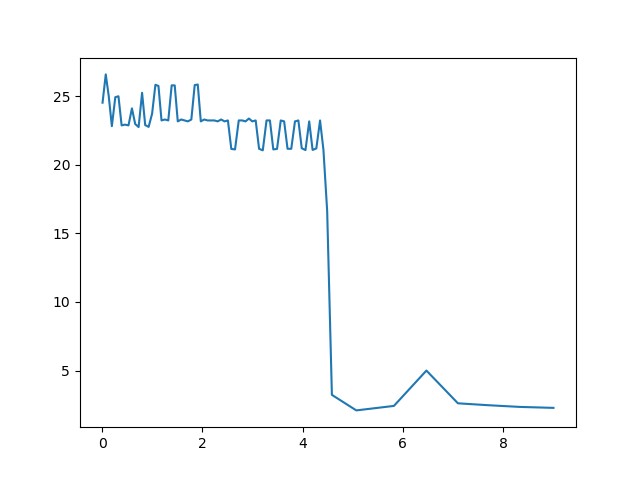
\includegraphics[width=\textwidth]{img/v-theta-4}
    \caption{The graph of the angular velocity of the fourth trial versus time}
    \label{fig:v-theta-4}
  \end{subfigure}
  \begin{subfigure}{.45\textwidth}
    \centering
    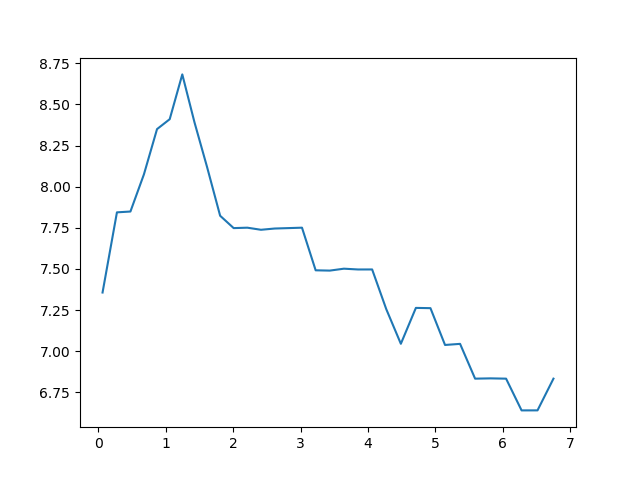
\includegraphics[width=\textwidth]{img/v-theta-2}
    \caption{The graph of the angular velocity of the second trial versus time}
    \label{fig:v-theta-2}
  \end{subfigure}
\end{figure}

\paragraph*{}
The angle of inclination was calculated by subtracting its maximum value from
its minimum value:
$$\Delta \psi = (\psi_{max} - \psi_{min}) \pm 2 \psi_{error}$$

\paragraph*{}
These calculations were done for all 10 trials. The results of these
calculations are given in table \ref{tbl:processed-data}.

\begin{table}[h!]
  \centering
  \begin{tabular}{c|c|c|c}
    $\omega \left[ \si{\frac{2 \pi}{s}} \right]$ & 
    $\psi \left[ \si{\degree} \right]$ & 
    $\Delta \omega \left[ \si{\frac{2 \pi}{s}} \right]$ & 
    $\Delta \psi \left[ \si{\degree} \right]$ \\ \hline \hline
    7.527 & 80.93 & 0.529 & 0.79 \\ \hline
    15.46 & 19.63 & 4.658 & 0.79 \\ \hline
    18.04 & 117.5 & 7.062 & 0.79 \\ \hline
    18.51 & 142.1 & 3.189 & 0.79 \\ \hline
    19.75 & 13.29 & 6.429 & 0.79 \\ \hline
    20.95 & 131.7 & 6.451 & 0.79 \\ \hline
    22.74 & 23.83 & 3.604 & 0.79 \\ \hline
    25.97 & 16.94 & 2.485 & 0.79 \\ \hline
    26.04 & 91.88 & 6.600 & 0.79 \\ \hline
    32.23 & 17.29 & 14.80 & 0.79 \\ \hline
  \end{tabular}
  \caption{The processed data}
  \label{tbl:processed-data}
\end{table}

\paragraph*{} Finally, a graph of the relationship between the average angular
velocity and the angle of inclination was plotted and is given in figure
\ref{fig:relationship}.

\begin{figure}[ht]
  \centering
  \begin{tikzpicture}
    \begin{axis}[
        xlabel={The angular velocity $ \omega \left[ \si{\frac{2 \pi}{s}} \right]$},
        ylabel={The angle of inclination $ \psi \left[ \si{\degree} \right]$}
      ]
      \addplot[
        mark=o,
        mark size = 0pt,
        only marks
      ]
        plot [
          error bars/.cd,
          x dir=both,
          x explicit,
          y dir=both,
          y explicit
        ]
        coordinates {
          (7.526592031289145,80.9326171875) +- (0.5285461493199469,0.7853981633974483)
          (15.462900816759667,19.62890625) +- (4.657548336099565,0.7853981633974483)
          (18.03740060637572,117.54557291666667) +- (7.062111867998039,0.7853981633974483)
          (18.512190251100144,142.1142578125) +- (3.189057382819494,0.7853981633974483)
          (19.752989343008,13.29345703125) +- (6.4293121659957855,0.7853981633974483)
          (20.945598090953492,131.70635516826923) +- (6.450927815029516,0.7853981633974483)
          (22.741657085201375,23.828125) +- (3.603729047077891,0.7853981633974483)
          (25.97397602256961,16.943359375) +- (2.4849756615744556,0.7853981633974483)
          (26.04316851590518,91.875) +- (6.6000940343773635,0.7853981633974483)
          (32.22822486490073,17.28515625) +- (14.084040448940591,0.7853981633974483)
        };
    \end{axis}
  \end{tikzpicture}
  \caption{The graph of the relationship between the angular velocity and the
  angle of inclination}
  \label{fig:relationship}
\end{figure}

\section{Analysis}

\paragraph*{}
It is obvious that graph \ref{fig:relationship} presents no correlation, even
though a clear correlation was expected. Moreover, the uncertainties over the
$x$ axis are extremely high, showing no useful information.

\paragraph*{}
Qualitative data (observing the mechanism), pointed to the angle of inclination
being lower for higher angular velocity, which the quantitative data does not
point to.

\section{Evaluation}

\paragraph*{}
Looking at the original graphs of the relationships between the angle of
inclination, the angular velocity and the angular path versus the time, shown
in figure \ref{fig:all-vs-time-5}, the reason behind the lack of correlation
becomes obvious.

\begin{figure}[ht]
  \centering
  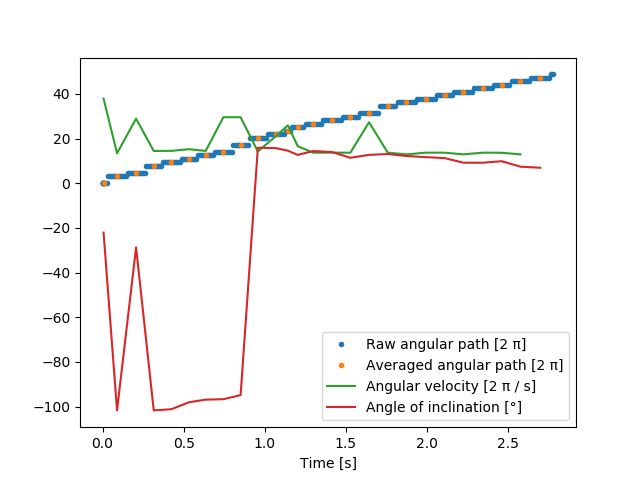
\includegraphics[width=0.7\textwidth]{img/all-vs-time-5}
  \caption{The graph of the angle of inclination, the angular velocity and the
  angular path versus time}
  \label{fig:all-vs-time-5}
\end{figure}

\paragraph*{}
Note how the graph of the angle of inclination behaves. Strangely, it does not
follow a linear trend as was qualitatively observed. This indicates that the
resistance of the potentiometer was not in proportion to the yaw of the gimbal.

\paragraph*{}
Since the potentiometer picked was a linear one, this indicates that a possible
reason for such inaccuracy could be that the potentiometer employed was broken.
Using a multimeter it was tested, and, as expected, it proved to read different
values without regard to the position of its axis.

\subsection{High uncertainty}

\paragraph*{}
The very high $x$ axis uncertainty is most likely a product of the \textit{reed
relay} not being fast enough to sense every time a magnet is in front of it.
This can be easily resolved by reducing the number of magnets on the wheel,
from $4$ to $1$.

\section{Conclusion}

\paragraph*{}
The experiment turned out extremely poorly. Due to malfunctioning measuring
equipment, the experiment did not shed accurate results. A further revision of
this experiment should address the malfunctioning potentiometer and remeasure
the data with operative equipment.

\paragraph*{}
The precision of the experiment was equally as poor. Counterintuitivelly, the
next revision of this experiment should reduce the number of magnets, so that
the \textit{reed relay} triggers with higher accuracy, increasing the precision
of the final graph.

\singlespacing
\pagebreak
\clearpage
\pagenumbering{gobble}
\section*{Works Cited}
\begin{hangparas}{.25in}{1}
  \begin{sloppypar}
    Arduino. \textit{Arduino Uno}. Farnell, 2019,
    \url{https://www.farnell.com/datasheets/1682209.pdf}. Accessed 17 Jan 2019.
    \\

    LucasVB. \textit{Image:3D\_Gyroscope.Png, But Without English Text}. 2006,
    \url{https://commons.wikimedia.org/wiki/File:3D_Gyroscope-no_text.png}.
    Accessed 16 Jan 2019. \\

    Python Software Foundation. \textit{Python Language Reference}. Version
    3.6. \\
  \end{sloppypar}
\end{hangparas}

\pagebreak
\section*{Appendix}

\subsection*{Raw data}

\tablefirsthead{ \toprule $T [\si{ms}] (\pm 1 \si{ms})$ & $N_{reed} [\text{ }]$
  & $Val_{pot} [\text{ }]$ \tabularnewline \midrule}

\tabletail{\midrule} \tablelasttail{\bottomrule}

\subsubsection*{Measurement 1}

\begin{multicols}{3}

  \TrickSupertabularIntoMulticols

  \begin{supertabular}{|c|c|c|}
    \csvreader[
      late after line=\\
    ]{../data/2weights/1.csv}{1=\time,2=\rev,3=\pot}{\time & \rev & \pot}
  \end{supertabular}

\end{multicols}

\pagebreak

\subsubsection*{Measurement 2}

\begin{multicols}{3}

  \TrickSupertabularIntoMulticols

  \begin{supertabular}{|c|c|c|}
    \csvreader[
      late after line=\\
    ]{../data/2weights/2.csv}{1=\time,2=\rev,3=\pot}{\time & \rev & \pot}
  \end{supertabular}

\end{multicols}

\pagebreak

\subsubsection*{Measurement 3}

\begin{multicols}{3}

  \TrickSupertabularIntoMulticols

  \begin{supertabular}{|c|c|c|}
    \csvreader[
      late after line=\\
    ]{../data/2weights/3.csv}{1=\time,2=\rev,3=\pot}{\time & \rev & \pot}
  \end{supertabular}

\end{multicols}

\pagebreak

\subsubsection*{Measurement 4}

\begin{multicols}{3}

  \TrickSupertabularIntoMulticols

  \begin{supertabular}{|c|c|c|}
    \csvreader[
      late after line=\\
    ]{../data/2weights/4.csv}{1=\time,2=\rev,3=\pot}{\time & \rev & \pot}
  \end{supertabular}

\end{multicols}

\pagebreak

\subsubsection*{Measurement 5}

\begin{multicols}{3}

  \TrickSupertabularIntoMulticols

  \begin{supertabular}{|c|c|c|}
    \csvreader[
      late after line=\\
    ]{../data/2weights/5.csv}{1=\time,2=\rev,3=\pot}{\time & \rev & \pot}
  \end{supertabular}

\end{multicols}

\pagebreak

\subsubsection*{Measurement 6}

\begin{multicols}{3}

  \TrickSupertabularIntoMulticols

  \begin{supertabular}{|c|c|c|}
    \csvreader[
      late after line=\\
    ]{../data/2weights/6.csv}{1=\time,2=\rev,3=\pot}{\time & \rev & \pot}
  \end{supertabular}

\end{multicols}

\pagebreak

\subsubsection*{Measurement 7}

\begin{multicols}{3}

  \TrickSupertabularIntoMulticols

  \begin{supertabular}{|c|c|c|}
    \csvreader[
      late after line=\\
    ]{../data/2weights/7.csv}{1=\time,2=\rev,3=\pot}{\time & \rev & \pot}
  \end{supertabular}

\end{multicols}

\pagebreak

\subsubsection*{Measurement 8}

\begin{multicols}{3}

  \TrickSupertabularIntoMulticols

  \begin{supertabular}{|c|c|c|}
    \csvreader[
      late after line=\\
    ]{../data/2weights/8.csv}{1=\time,2=\rev,3=\pot}{\time & \rev & \pot}
  \end{supertabular}

\end{multicols}

\pagebreak

\subsubsection*{Measurement 9}

\begin{multicols}{3}

  \TrickSupertabularIntoMulticols

  \begin{supertabular}{|c|c|c|}
    \csvreader[
      late after line=\\
    ]{../data/2weights/9.csv}{1=\time,2=\rev,3=\pot}{\time & \rev & \pot}
  \end{supertabular}

\end{multicols}

\pagebreak

\subsubsection*{Measurement 10}

\begin{multicols}{3}

  \TrickSupertabularIntoMulticols

  \begin{supertabular}{|c|c|c|}
    \csvreader[
      late after line=\\
    ]{../data/2weights/10.csv}{1=\time,2=\rev,3=\pot}{\time & \rev & \pot}
  \end{supertabular}

\end{multicols}

\pagebreak

\subsection*{Arduino Uno code}
\lstinputlisting[frame=single, language=C]{../TorqueMeasurer/TorqueMeasurer.ino}

\subsection*{Data Processing code}
\lstinputlisting[frame=single, language=python]{../plot.py}

\end{document}

